\documentclass[a4paper,UKenglish,cleveref]{lipics-v2019}

\usepackage[utf8]{inputenc}
\usepackage{amsmath}
\usepackage{amsfonts}
\usepackage{amssymb}
\usepackage{amsthm}
\usepackage{graphicx}
\usepackage{wrapfig}
\usepackage{makecell}
\usepackage{xspace}
\usepackage[usenames,dvipsnames]{xcolor}
\usepackage{caption}
\usepackage{wrapfig}
\usepackage{float}
\usepackage{booktabs}
%\usepackage[margin=0.7in,footskip=0.25in]{geometry}

%\newtheorem{definition}{Definition}
\newtheorem{condition}{Condition}
\newtheorem{conjecture}{Conjecture}
\newtheorem{observation}{Observation}
%\newtheorem{lemma}{Lemma}
%\newtheorem{theorem}{Theorem}

\newcommand{\mremark}[3]{\textcolor{blue}{\textsc{#1 #2:}} \textcolor{SeaGreen}{\textsf{#3}}}

\newcommand{\frank}[2][says]{\mremark{Frank}{#1}{#2}}
\newcommand{\maarten}[2][says]{\mremark{Maarten}{#1}{#2}}
\newcommand{\marc}[2][says]{\mremark{Marc}{#1}{#2}}
\newcommand{\jerome}[2][says]{\mremark{J\'er\^ome}{#1}{#2}}
\newcommand{\jordi}[2][says]{\mremark{Jordi}{#1}{#2}}
\newcommand{\ivor}[2][says]{\mremark{Ivor}{#1}{#2}}
\newcommand{\mees}[2][says]{\mremark{Mees}{#1}{#2}}
\newcommand{\todo}[2][DO]{\mremark{TO}{#1}{#2}}
\newcommand{\draw}{\todo{draw}}

\newcommand{\bigo}{\ensuremath{\mathcal O}}

\newcommand{\spg}{\mathcal{S\!P}}
\newcommand{\ixi}{\mathcal{I}}
\newcommand{\pix}{\square}
\newcommand{\spix}{\boxplus}

\newcommand{\eps}{\varepsilon}
\newcommand{\R}{\mathbb{R}}

\title{Pixelating Polygons}
\begin{document}
\maketitle

\section{Introduction}

Given a set of disjoint simply connected regions $\cal R$, we wish to assign each $R \in \cal R$ to a grid polygon $P$ (defined formally in Section~\ref {sec:prelims}) which represents $R$.

%We focus on the case where each $R$ is a simple polygon.
\maarten {I dropped the assumption that the input regions are polygons - all our combinatorial bounds also apply to the case where $R$ is any simply connected region (i.e. its boundary is a closed curve, but not necessarily polygonal). We also don't have any bounds that depend on the number of vertices of $R$. It makes a difference when we want to actually compute the pixel polygons, but I think we will not focus on that, and when we do make a remark about it we can simply say that the remark applies to the case where the regions are polygonal.  Finally, it makes the choice of letters more logical, we can use $P$ for the output Pixel-Poligon. :)}

%To successfully map a disjoint hole $R_i$ we need to outline its border as a disjoint cycle of black cells.

%Now suppose that for two holes $R_1, R_2 \in H$ their border is present in the same cell $\pix \in G$. We could color the cell black, and say that the pixel is part of both the border of $R_1$ and of $R_2$. But in this case, the holes $R_1$ and $R_2$ intersect one another, whereas in the original drawing $A$ this was not the case. The only option that we have, is to stretch and transpose $A$, such that only one of the two holes has its border in $\pix$.

One way to measure how much we needed to "stretch" the original polygons is to measure the symmetrical Hausdorff distance between $R_i$ and its mapping $P_i$.
We require that the Hausdorff distance between the boundaries of the polygons is limited and also that the Hausdorff distance between the points inside the polygons is limited.
Let $\eps$ be the maximum allowed Hausdorff distance, called \emph{similarity}.
%\maarten {What is the intuition behind the use of the word "stretch" here? I would juse say "similarity" (or distance, or something like that).}

\iffalse
Formally this means: $\forall i\in \{1, m\}$
\begin{itemize}
	\item $\forall s\in \partial R_i, \exists t\in \partial P_i, |st|\leq \eps$
	\item $\forall s\in \partial P_i, \exists t\in \partial R_i, |st|\leq \eps$
	\item $\forall s\in  R_i, \exists t\in  P_i, |st|\leq \eps$
	\item $\forall s\in  P_i, \exists t\in  R_i, |st|\leq \eps$
\end{itemize}
where $|\cdot|$ denotes Euclidean distance.
\fi

The goal of this paper is to find a mapping where the similarity is asymptotically minimized. In this work we look at different types of polygons and the theta-bounds on the Hausdorff distance. See the table below for a summary of the results.
See Figure \ref{fig:pixelexample} for an example.

%\begin{definition}
%Suppose $H$ is a collection of holes $R_1 ... R_m$. Let $b_1 ... b_m$ be the borders of $R_1 ... R_m$ and let $f(H)$ be the projection of $H$ onto the grid.

%We say the projection $f$ is \textbf{valid} if there is a bijection $g$ between $\{ b_1 ... b_m \}$ and a set of disjoint black cycles in $f(H)$.
%\end{definition}

%\begin{lemma}
%\label{lemma:expand}
%\jerome{This is wrong!!!} \jerome{It is rather that for each grid polygon that we create, this holds.}
%Let $H$ be a collection of holes. If there exists a valid projection $f$, where for each border $b_i$, the symmetrical Hausdorff distance between $b_i$ and $g(b_i)$ is $\Theta( X)$, then the symmetrical Hausdorff distance between $H$ and $f(H)$ is $\Theta(X)$.
%\end{lemma}

%This lemma allows us to focus on only projecting the boundaries of a hole.


%\begin{figure}[H]
%\centering
%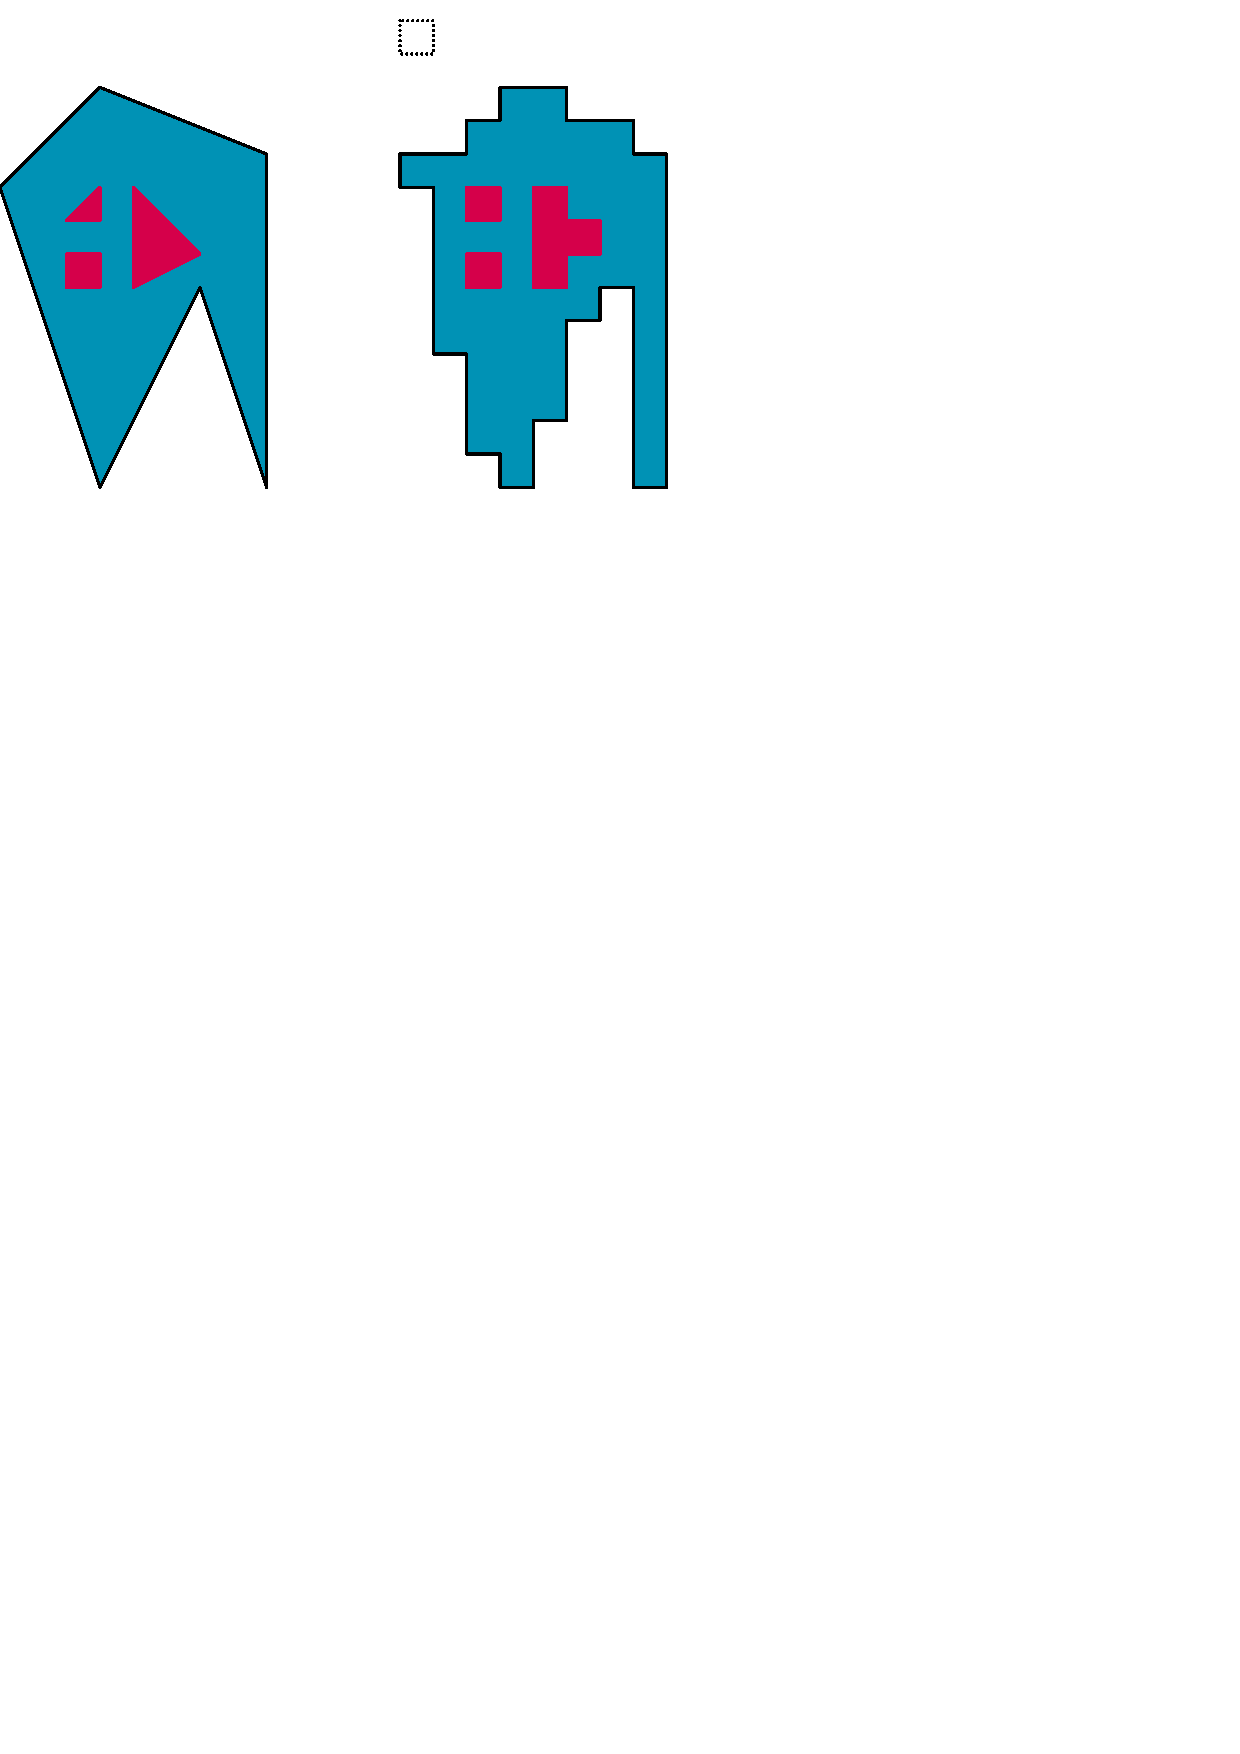
\includegraphics[width=150px]{Figures/pixelexample.pdf}
%\caption{\jerome{redo}
%Left is $A$: A simple polygon with $m=3$ holes. To the right is the projection $B$ to pixels with diameter $d$ with a symmetrical Hausdorff distance less than $2*d$.
%}
%\label{fig:pixelexample}
%\end{figure}




\begin{table}[H]
\begin{tabular}{lcc}
\toprule
Restrictions on the regions & Lower bound & Upper bound  \\ \midrule
point regions & $\Omega(\sqrt[]{m}) $ & $\bigo(\sqrt[]{m})$ \\
$\beta$-fat regions & $\Omega(\sqrt[]{m}) $ & $\bigo(\sqrt[]{m})$ \\
convex regions & $\Omega(m) $ & $\bigo(m)$ \\
two unrestricted regions &  $\Omega(1)$ & $\bigo(1)$\\
three unrestricted regions &  \multicolumn{2}{c}{unbounded}\\
\bottomrule
%$\Omega(2^m)$ & $\bigo(2^m)$ \\ \hline
\end{tabular}
\end{table}


\section{Preliminaries}
\label {sec:prelims}

\subparagraph {Simple grid polygons.}

Let $\Xi$ be the (infinite) unit grid, which we interpret as a set of {\em pixels} (unit squares):
an element $\pix \in \Xi$ is a subset of $\R^2$ of the form $[a,a+1]\times[b,b+1]$ for integers $a$ and $b$.
For a given set of pixels $X \subset \Xi$, we denote the region $\cup_{\pix \in X}\pix$ covered by $X$ simply by $\cup(X)$, and we write $\partial(X)$ for the boundary of $\cup(X)$.

\jordi{I personally find the symbols we use (square, cup) a bit annoying. It seems to make more sense to have $\xi \in \Xi$, and I think the convention is to just write $\partial P$ for the boundary of $P$. Also, do we need to differentiate between a set of pixels $X$ and the region it covers? I.e. can't we just use $X$ to denote the region?}

\begin{definition}
A {\em simple grid polygon} $P = \cup(X)$ is the union of a set of pixels $X \subset \Xi$ for which $\partial(X)$ is a single, simple closed curve.
\end{definition}

\maarten {Not sure we need the following definitions.}

\begin{definition}
Two pixels are \emph{adjacent} iff they share a side.
\end{definition}

Adjacency induces the graph $G=(\Xi, E)$ with $(v, w)\in E \iff v$ and $w$ are adjacent.
For $v\in \Xi$, let $N(v)$ be the four neighbors of v. Further for $W\subseteq \Xi$, let $N(W)=\bigcup_{v\in W} N(v)$.

\subparagraph {Similarity.}

The {\em Hausdorff distance}~\cite{} between two sets $A, B \subset \R^2$ is defined as
\[
  H(A, B) = \max \{\max_{a \in A}(\min_{b \in B}(|ab|)), \max_{b \in B}(\min_{a \in A}(|ab|))\}
\]

Note that the Hausdorff distance between any two closed sets is equal to the Hausdorff distance between the boundaries of those sets.

Let $R$ be a simply connected region, and let $P$ be a simple grid polygon.

\begin{definition}
We define $R$ and $P$ to be {\em $\eps$-similar} if $H(R,P) \le \eps$.
\end{definition}


\subparagraph {Problem statement.}

Consider a set of $m$ disjoint simply-connected regions $\mathcal{R} = \{R_1, R_2, \ldots, R_m\}$ in $\mathbb{R}^2$.
We wish to assign to each $R_i$ a simple grid polygon $P_i$ such that $P_i$ is $\eps$-similar to $R_i$ and $P_i\cap P_j=\emptyset$.
We further require that the grid polygons are sufficiently spaced; that is, $\partial(P_i) \cap \partial(P_j) = \emptyset, \forall i \ne j$. \maarten {Do we? Or do we only require the actual sets of pixels to be disjoint? It doesn't really matter, so what we do depends on the story we tell in the introduction, I think.}\jerome{Each of our algorithms produces such a result, i.e., that the boundaries do no touch.}
\marc{I added that the grid polygons must be disjoint. This by definition implies that they cannot touch; they are closed objects. So we can remove the spacing requirement.}
When this is the case, we also say that the set of grid polygons $\mathcal{P} = \{P_1, P_2, \ldots, P_m\}$ is {\em $\eps$-similar} to $\cal R$.

The question we are concerned with is: for a given class of regions (i.e.\ points, fat regions, convex regions, general regions) and a given number $m$, what is the smallest value $\eps$ such that for any set of $m$ regions from the class, there always exists an $\eps$-similar set of $m$ grid polygons?

\maarten {The following is an equivalent interpretation of the problem, which could help with the intuition and/or be used in the technical sections. If we don't use it, we might not want to define it.}

We may interpret a solution as a {\em coloring} of $\Xi$ in the following way.
Each pixel $\pix\in\Xi$ can only be assigned one color. The set of colors is $C = \{c_1,\dots c_m\}\cup\{b\}$, where $c_i$ is the color of the input region $R_i$ and $b$ is the background color.
Formally the coloring is then a map $f:\Xi\to C$.
Let ${\cal P}_f=\{P_1,\dots, P_m\}$ or short ${\cal P}$ be the set of grid polygons induced by $f$.

\begin{definition}
A coloring is \emph{valid}, iff the following holds:
\begin{enumerate}
	\item When two adjacent pixels have a different color, then one of them must be $b$. That way no two polygons touch. \marc{Except for vertex-adjacency.}
	\item For each region $R_i$ the pixels colored $c_i$ is simple. Let $P_i$ be the polygon formed by those pixels.
	\item The polygon $P_i$ formed by the pixels colored does not contain holes.
\end{enumerate}

\jordi{Does 2 not imply 3? A simply connected region cannot have holes.}

%If we want to use the same definition as Bouts~\emph{et al.}, we also request that the pixels on the boundary of $P_i$ form a simple cycle without chords. Informally this means that $P_i$ does not contain holes.
%\jerome{But that way we can have a rectangle + one pixel, because the boundary is then a cycle with a leaf\dots (???)}
\end{definition}


\subparagraph {Superpixels.}

The following concepts will be useful.

For any positive integer $k$, let $k\Xi$ be the unit grid scaled by a factor $k$, that is, the grid consisting of squares of the form $[ka, ka+k] \times [kb, kb+k]$ for integers $a, b$.

\begin{definition}
%In all of the following chapters we use the following notion:
A \emph{superpixel} $\spix$ of size $k^2$ is a set of $k^2$ pixels in $\Xi$ whose union is a square in $k\Xi$. %A superpixel grid of size $k^2$ is a set $k\Xi$ of superpixels of length $k$ each such that the following holds:
%(1) each pixel is in exactly one superpixel,(2) the superpixels are aligned, i.e., $\forall \spix_1, \spix_2\in k\Xi, |N(\spix_1)\cap \spix_2| \in \{0, k\}$.
\end{definition}

\jordi{using $\spix$ as the symbol makes me think these are smaller than the original pixels...}

\maarten {I simplified the definition by fixing the alignment of a superpixel grid. I think that should be fine and we never need to shift the grid (do we?), but be careful with arguments about superpixel grids.}

The superpixels induce the graph $G$ in the same way that the pixels induce $G$.

%For a pixel $\pix$ we denote by $a(\pix)\in \mathbb{R}$ the set of points covered by $\pix$.
%\maarten {Not necessary, right now a pixel *is* the set of points covered by it.}
For a superpixel $\spix$ we denote by $\cup(\spix)$ the union of the pixels in the set, that is, the set of points covered by the pixels in $\spix$.
%\maarten {The following is kind of obvious, remove?}
%A region $R$ \emph{intersects} (super)pixel $o$ if $R\cap \cup(o)\neq \emptyset$. A polygon $R$ \emph{contains} (super)pixel $o$ if $\cup(o)\subseteq R$.

\begin{definition}
For a fixed $i\in \{1, m\}$ and a valid coloring $f$ of $\cal R$ using the pixels of $\Xi$ and a given superpixel grid $k\Xi$, the polygon $P_i$ \emph{respects} $k\Xi$, if the following holds for each $\spix\in k\Xi$:
\begin{enumerate}
	\item if $R_i$ contains a superpixel, then so does $P_i$ and vice-versa,
	\item if $R_i$ intersects a superpixel, then so does $P_i$ and vice-versa.
\end{enumerate}
\end{definition}

\jordi{We need to be careful with the definition of containment here, i.e. if a superpixel is considered contained even with its vertices on the boundary of the region, our algorithm for convex regions gives an output that does not respect the superpixel grid.}

\begin{lemma}\label{lem:respect_means_bound}
Let $\cal R$ be a set of input regions, $\Xi$ be the unit grid and $k\Xi$ a superpixel grid of size $k^2$. Further let $f$ be a valid coloring of $\cal R$ using the pixels of $\Xi$.
If each polygon in ${\cal P}_f$ respects $k\Xi$, then the similarity of the coloring is at most $\sqrt{2}k$.
\end{lemma}
The proof follows by definition.

\jordi{I guess the "grid of size $k^2$" means cells that are $k \times k$. This seems to follow from the definition of $k\Xi$. Adding this statement here makes it sound like we have a grid of $k \times k$ superpixels.}

\section{Input regions are points.}
\label{sec:points}
By examining the problem under the constraint that all input regions are points, we can see that even for the simplest possible regions it is not possible to bound the Hausdorff distance to a constant factor.

%TL;DR

%lower bound:
%place them all within one pixel

%upper bound: worst case optimal algorithm

%overlay everything with superpixels, and then place pixels at random

\subsection{Lower Bound}
\label{sub:points_lower}
The worst-case lower bound on the similarity when all the regions in \(\cal R\) are points is \(O(\sqrt{m})\). To see why this is true consider the case where all of the regions (points) are located within the same unit square. Since each point must be assigned it's own disjoint region consisting of at least 1 pixel, a set \(X \subset \Xi\) around this square with \(\cup(X)=4m\) is needed to assign each point a pixel. The distance from \(\partial(X)\) to its center, i.e. the square containing the input regions, is then \(O(\sqrt{m})\).

% subsection points_lower (end)

\subsection{Constructive Upper Bound}
\label{sub:points_upper}
We will now sketch an algorithm that realizes a worst-case similarity of \(O(\sqrt{m})\) in the case where the regions are points. Showing that our lower bound is tight.

We start by overlaying \(\Xi\) on \(\cal R\). We then create a superpixel \(\spix_i\) for each \(R_i \in \cal R\) with size \((2\sqrt{m})^2\). We place these superpixels such that the pixel containing \(R_i\) is in the center of \(\spix_i\) (the superpixels may overlap). We then iteratively assign each region \(R_i\) their grid polygon \(P_i\), which consists of a single pixel contained somewhere in \(\spix_i\) that is disjoint from all previously assigned polygons. Since each superpixel contains \(4m\) pixels there must always be a pixel we can choose for this, and the assigned pixels have Hausdorff distance \(O(\sqrt{m})\) to the input region. 

% subsection points_upper (end)

%\subsection{(Algorithm)}
\label{sub:points_algo}



% subsection points_algo (end)



% section points (end)

\section{Input regions are convex $\beta$-fat regions.}
\label{sec:fat}
TL;DR

lower bound

same as above

upper bound

overlay everything with superpixels:
\begin{enumerate}
	\item if a SP is completely covered $\rightarrow$ color
	%\item for each poly that has superpixels, but they are not connected, connect them using SPs where the poly is present
	\item then for each poly not yet present at all: choose random pixel in a SP where you are.
\end{enumerate}
This means Lemma~\ref{lem:respect_means_bound} is not completely fulfilled. We did not make sure that each polygon $P_i$ is present in each SP that $R_i$ intersects. But due to the fatness, we know that we are at least present in a ~close-by SP. We just have to prove that this is a constant and then we are done using a proof similar to the lemma.


(Note that if the regions are not convex, then the polygons could be disconnected.)


\subsection{Lower Bound}
\label{sub:fat_lower}



% subsection fat_lower (end)

\subsection{Constructive Upper Bound}
\label{sub:fat_upper}



% subsection fat_upper (end)

\subsection{(Algorithm)}
\label{sub:fat_algo}



% subsection fat_algo (end)


% section fat (end)

\section{Input regions are convex regions.}\label{sec:convex}
\subsection{Lower Bound}\label{sub:convex_lower}

Let the regions have as their only requirement that they are convex. In that case we can immediately show that the coloring has a lower-bound Hausdorff distance of $\Theta(m)$. The construction is shown in Figure \ref{fig:linesexample}.

\begin{figure}
\centering
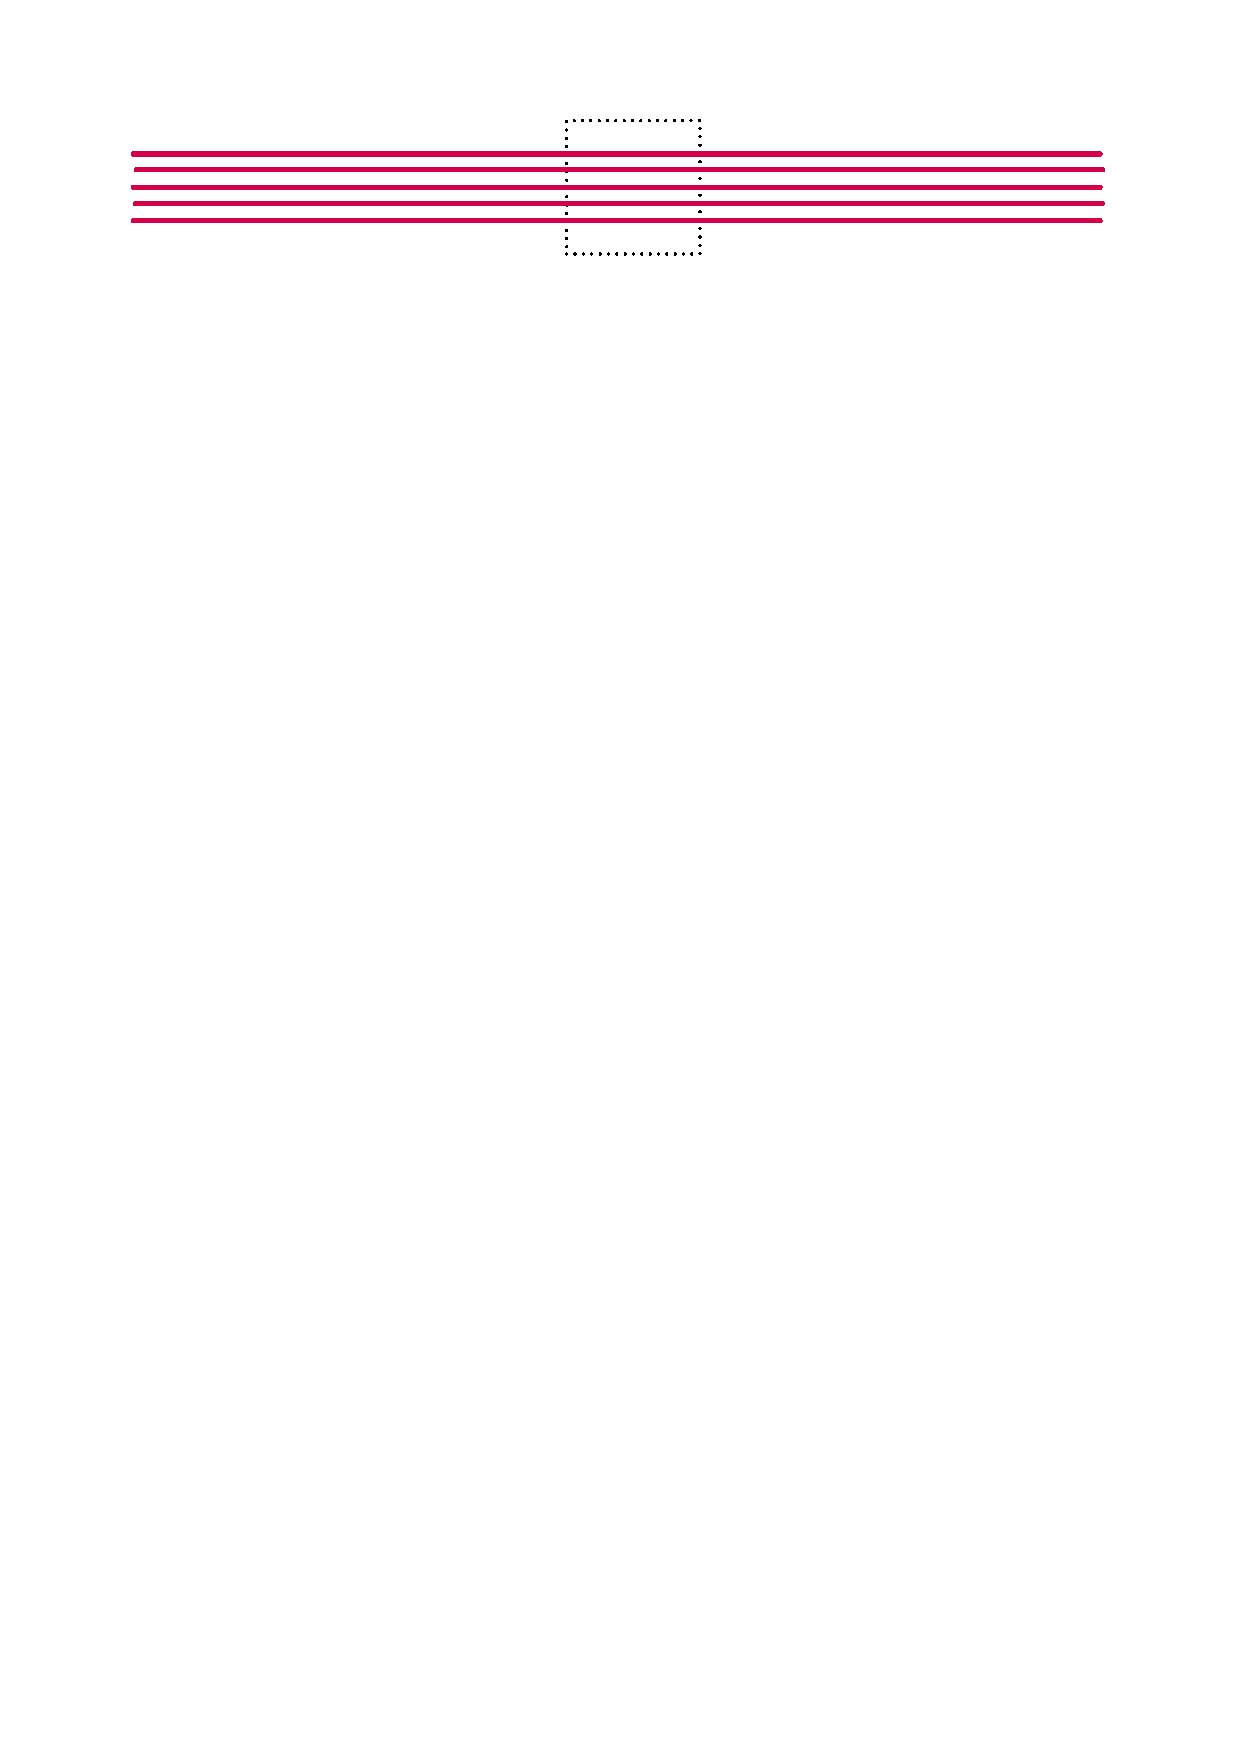
\includegraphics[scale=0.8]{Figures/linesexample.pdf}
\caption{The dotted square is a pixel. We can let $m$ vertical lines intersect the pixel. If their length is far greater than $m$, we can only project these regions to $m$ disjoint lines of pixels, which means that the outer lines must have a Hausdorff distance of $\Theta(m)$.}
\label{fig:linesexample}
\end{figure}


% subsection convex_lower (end)

\subsection{Constructive Upper Bound}
\label{sub:convex_upper}
We will describe an algorithm that, given a set of convex regions \(\mathcal{R}\), gives a set of orthoconvex grid polygons \(\mathcal{P}\) such that \(\mathcal{R}\) and \(\mathcal{P}\) are \(\Theta(m)\)-similar.

\begin{observation}\label{obs:convex-ordering}
Let \(R_1,R_2 \in \mathcal{R}\) be two convex regions. A horizontal line that intersects both regions will have them appear in a certain left-to-right order. There cannot be another horizontal line where this order is reversed. A symmetrical property holds for vertical lines, where there is a top-to-bottom order.
\end{observation}

\cref{obs:convex-ordering} allows us to define two partial orders \(\preceq_x\) and \(\preceq_y\) on \(\mathcal{R}\): \(R_i \preceq_x R_j\) iff the leftmost point in \(R_i\) does not lie to the right of the leftmost point in \(R_j\), and \(R_i \preceq_y R_j\) iff the topmost point in \(R_i\) does not lie below the topmost point in \(R_j\). Now let \(X_\mathcal{R}\) and \(Y_\mathcal{R}\) be two indices on \(R\) that respect \(\preceq_x\) and \(\preceq_y\), respectively, and let \(k\Xi\) be a superpixel grid with \(k = 2m\). Finally, for any superpixel \(\spix \in k\Xi\), we denote by \(\spix[x, y]\) the pixel that is the \(2x\)th from the left and \(2y\)th from the top within \(\spix\).

Our algorithm works as follows:

\begin{enumerate}
	\item For each superpixel \(\spix\) that is intersected by a region \(R_i\), we color \(\spix[X_\mathcal{R}(R_i), Y_\mathcal{R}(R_i)]\) with \(c_i\).
	\item For any two pixels that are colored with \(c_i\) in adjacent superpixels, we color all pixels on the straight line segment between them with \(c_i\) as well.
	\item For any four superpixels that form a cycle in \(G\), if they each contain a pixel colored with \(c_i\) in Step 1, we color all pixels in the square between these pixels with \(c_i\) as well.
\end{enumerate}

\noindent
See \cref{fig:convexprojection} for an illustration.

\begin{figure}
\centering
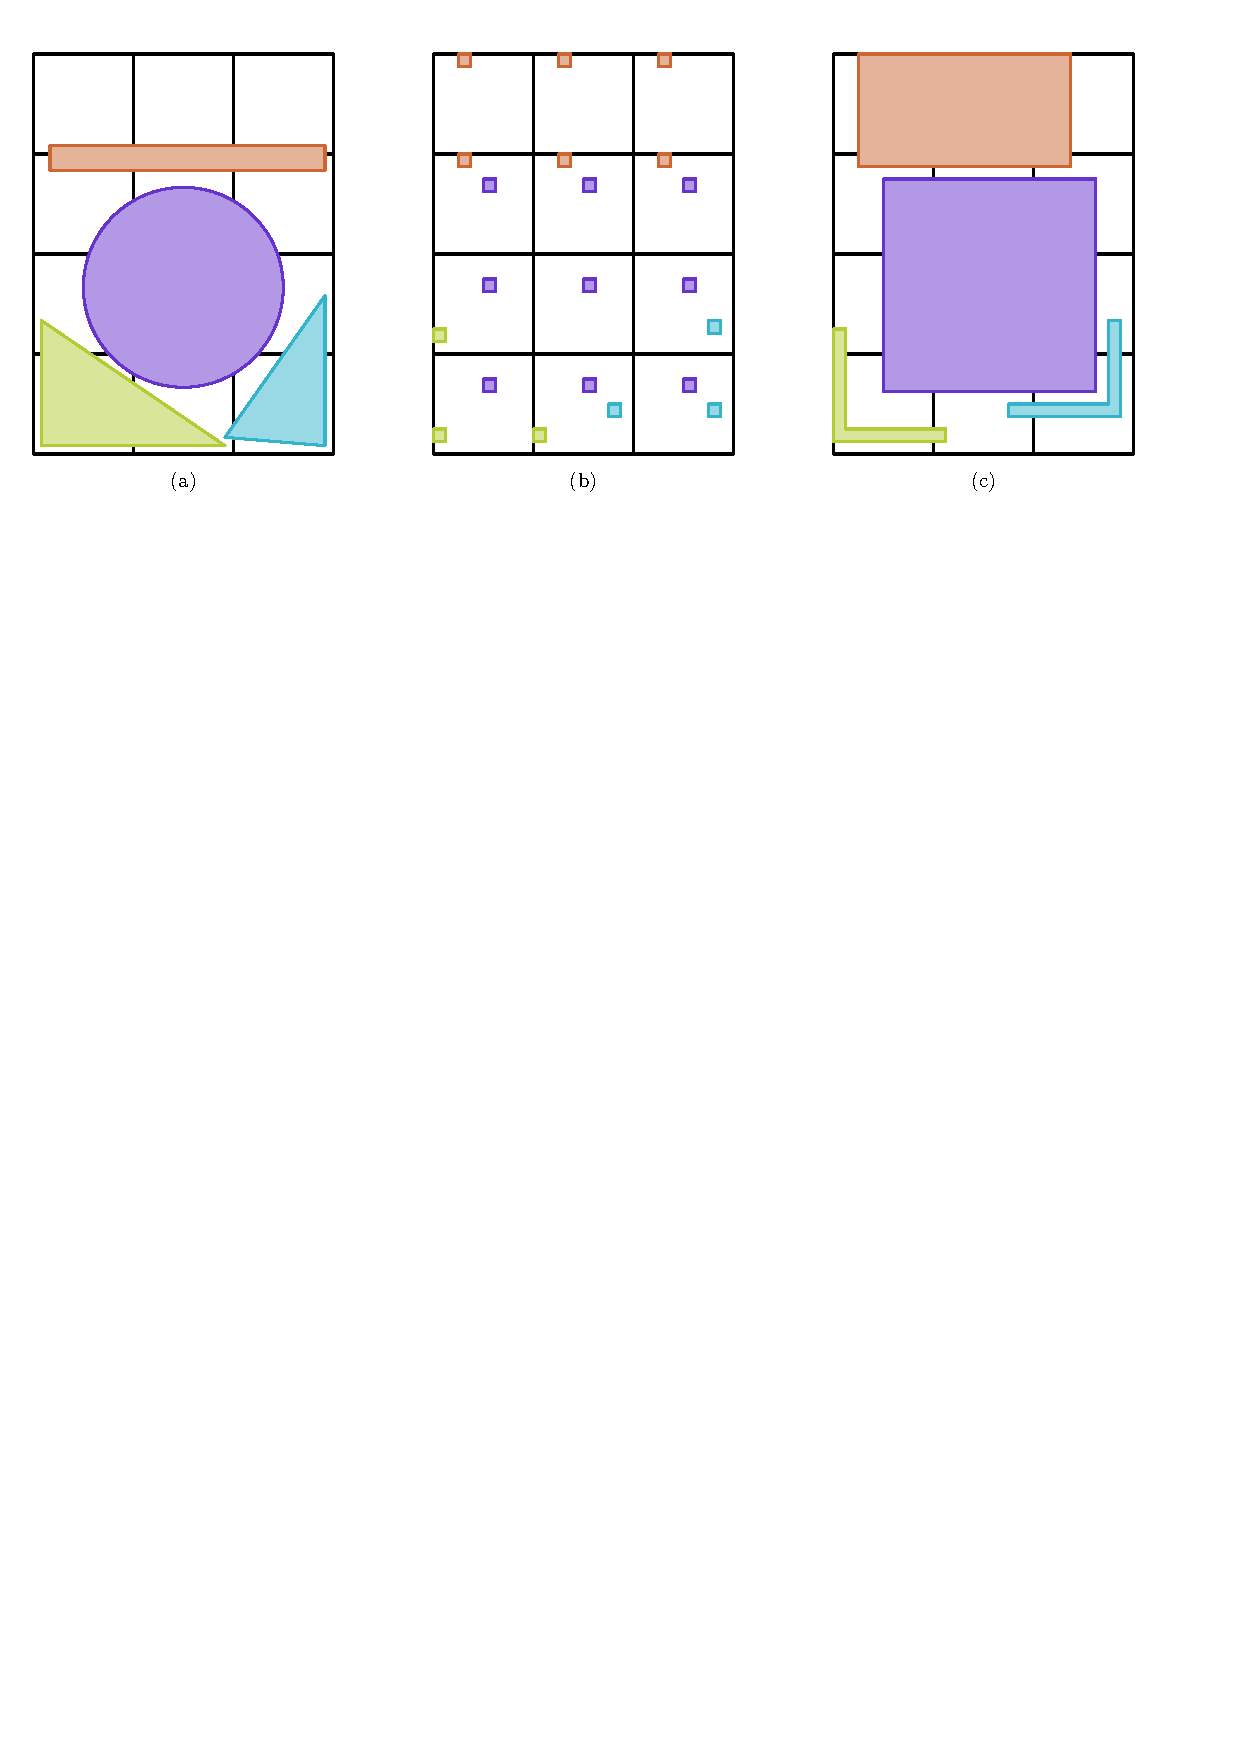
\includegraphics[width=\textwidth]{Figures/convexprojection.pdf}
\caption{The coloring algorithm for convex regions. (a) shows the input of four convex regions, overlaid onto a superpixel grid with \(k = 8\). (b) shows the pixels colored in Step 1 of the algorithm. (c) shows the final coloring obtained after Steps 2 and 3.}
\label{fig:convexprojection}
\end{figure}

Let \(f\) be the coloring obtained by the algorithm above.

\begin{lemma}\label{lem:convex-simply-connected}
	The polygons induced by \(f\) are simply connected.
\end{lemma}
\begin{proof}
	Consider a polygon \(P_i\) induced by \(f\). Its connectedness follows directly from the connectedness of the polygons in the input: \(R_i\) must intersect a connected set of superpixels, and our algorithm connects all of these together. It also cannot contain holes: the presence of a hole would imply that the set of superpixels intersected by \(R_i\) contains a hole, which is not possible due to \(R_i\) being simply connected and convex.
\end{proof}

\begin{lemma}\label{lem:convex-separated}
	The polygons induced by \(f\) are separated by the background color.
\end{lemma}
\begin{proof}
	The coloring obtained in Step 1 is separated by construction; it remains to be shown that the pixels colored in Steps 2 and 3 are also separated.

	In Step 2, we only color horizontal and vertical sequences of pixels, and as each color has a unique row and column in each superpixel, it suffices to show that a horizontal sequence of color \(c_i\) never intersects a vertical sequence of color \(c_j\). Assume that two such sequences do intersect; there must be one superpixel \(S\) in which both colors are present. From \(S\), the horizontal sequence extends to the superpixel to the left or right, and the vertical sequence extends to the superpixel above or below. Assume w.l.o.g. one color appears in pixel \(S[x,y]\) and extends to the right, and that another color appears in pixel \(S[u,v]\) and extends downward (the other cases are symmetrical).

	As the sequences intersect, we have that \(x \leq u\) and \(v \leq y\). This implies that \(R_i \preceq_x R_j\) and \(R_j \preceq_y R_i\); note that either of these orders needs to be strict, otherwise \(R_i\) and \(R_j\) intersect. This means that either \(R_i\) contains a point strictly to the left of the leftmost point of \(R_j\), and \(R_j\) crosses from above \(R_i\) to below, or \(R_j\) contains a point strictly above the topmost point of \(R_i\), and \(R_i\) crosses from the left of \(R_j\) to the right. Both cases imply that \(R_i\) and \(R_j\) intersect, which contradicts our assumptions on the input. We conclude that no horizontal and vertical sequence can intersect, and that therefore Step 2 maintains the separation of colors.

	For Step 3 to cause an intersection, we would need to have a pixel \(S[x,y]\) with color \(c_i\) inside a region being filled with color \(c_j\). Let \(S[u,v]\) be the pixel in \(S\) with color \(c_j\); assume w.l.o.g. that \(x > u\) and \(y > v\) (again, the other cases are symmetrical). For an intersection to occur, we must be filling a square with color \(c_j\) to the bottom right from \(S[u,v]\). By the same argument as used for Step 2, this means that \(R_j\) crosses from the top or left of \(R_i\) to the right or bottom, which is only possible if \(R_i\) and \(R_j\) intersect.

	We conclude that none of the steps in the algorithm can violate the separation of the colors in \(f\), which implies that the induced polygons are separated by the background color.
\end{proof}

\begin{theorem}
	The polygons \(\mathcal{P}\) induced by \(f\) are \(\Theta(m)\)-similar to \(\mathcal{R}\).
\end{theorem}
\begin{proof}
	By \cref{lem:convex-simply-connected,lem:convex-separated}, \(f\) is a valid coloring. By construction, \(P_i\) intersects any superpixel that \(R_i\) does. Furthermore, any \(R_i\) that contains a superpixel \(S\) necessarily intersects all surrounding superpixels. As such, \(S\) will be completely filled with color \(c_i\) in Step 3 of the algorithm, implying that \(P_i\) also contains \(S\). These two facts combined imply that \(f\) respects the superpixel grid, which lets us apply \cref{lem:respect_means_bound} to obtain the bound.
\end{proof}

% subsection convex_upper (end)

% section convex (end)

\section{Arbitrary input regions.}
\label{sec:arbitrary}

\subsection{Two Polygons}

Refer to the paper "The painter’s problem: covering a grid with colored connected polygons".
Spoiler: we can pixelize two polygons at the same time using a constant stretch.

\subsection{Three of More Polygons}

\begin{theorem}\label{thm:unbouded}
% The amount of stretch needed to color a screen with three or more polygons is unbounded.
% There are instances of three polygons that can not be ... with
For each $\eps$ there exists an instance $\mathcal{R}=\{R_1, R_2, R_3\}$, such that there are no $\eps$-similar grid polygons.
\end{theorem}
\begin{proof}
%Assume that the stretch needed to color a screen with three polygons is bounded by $k$.
Assume that there is an $\eps$, such that each instance $\mathcal{R}=\{R_1, R_2, R_3\}$ allows $\eps$-similar grid polygons. Let $k=\left \lceil \eps \right \rceil$.

Now let $R_1$, $R_2$ and $R_3$ be three regions defined as follows:
\jerome{spiral that loops around $k$ times, see Figure~\ref{fig:arbitrary-spirals}}
The three regions are colored in $c_1$ (red), $c_2$ (green) and $c_3$ (blue).
Let $\ixi$ be the region containing all points that are within distance $k$ of two different regions $R_i$.

\begin{figure}
\centering
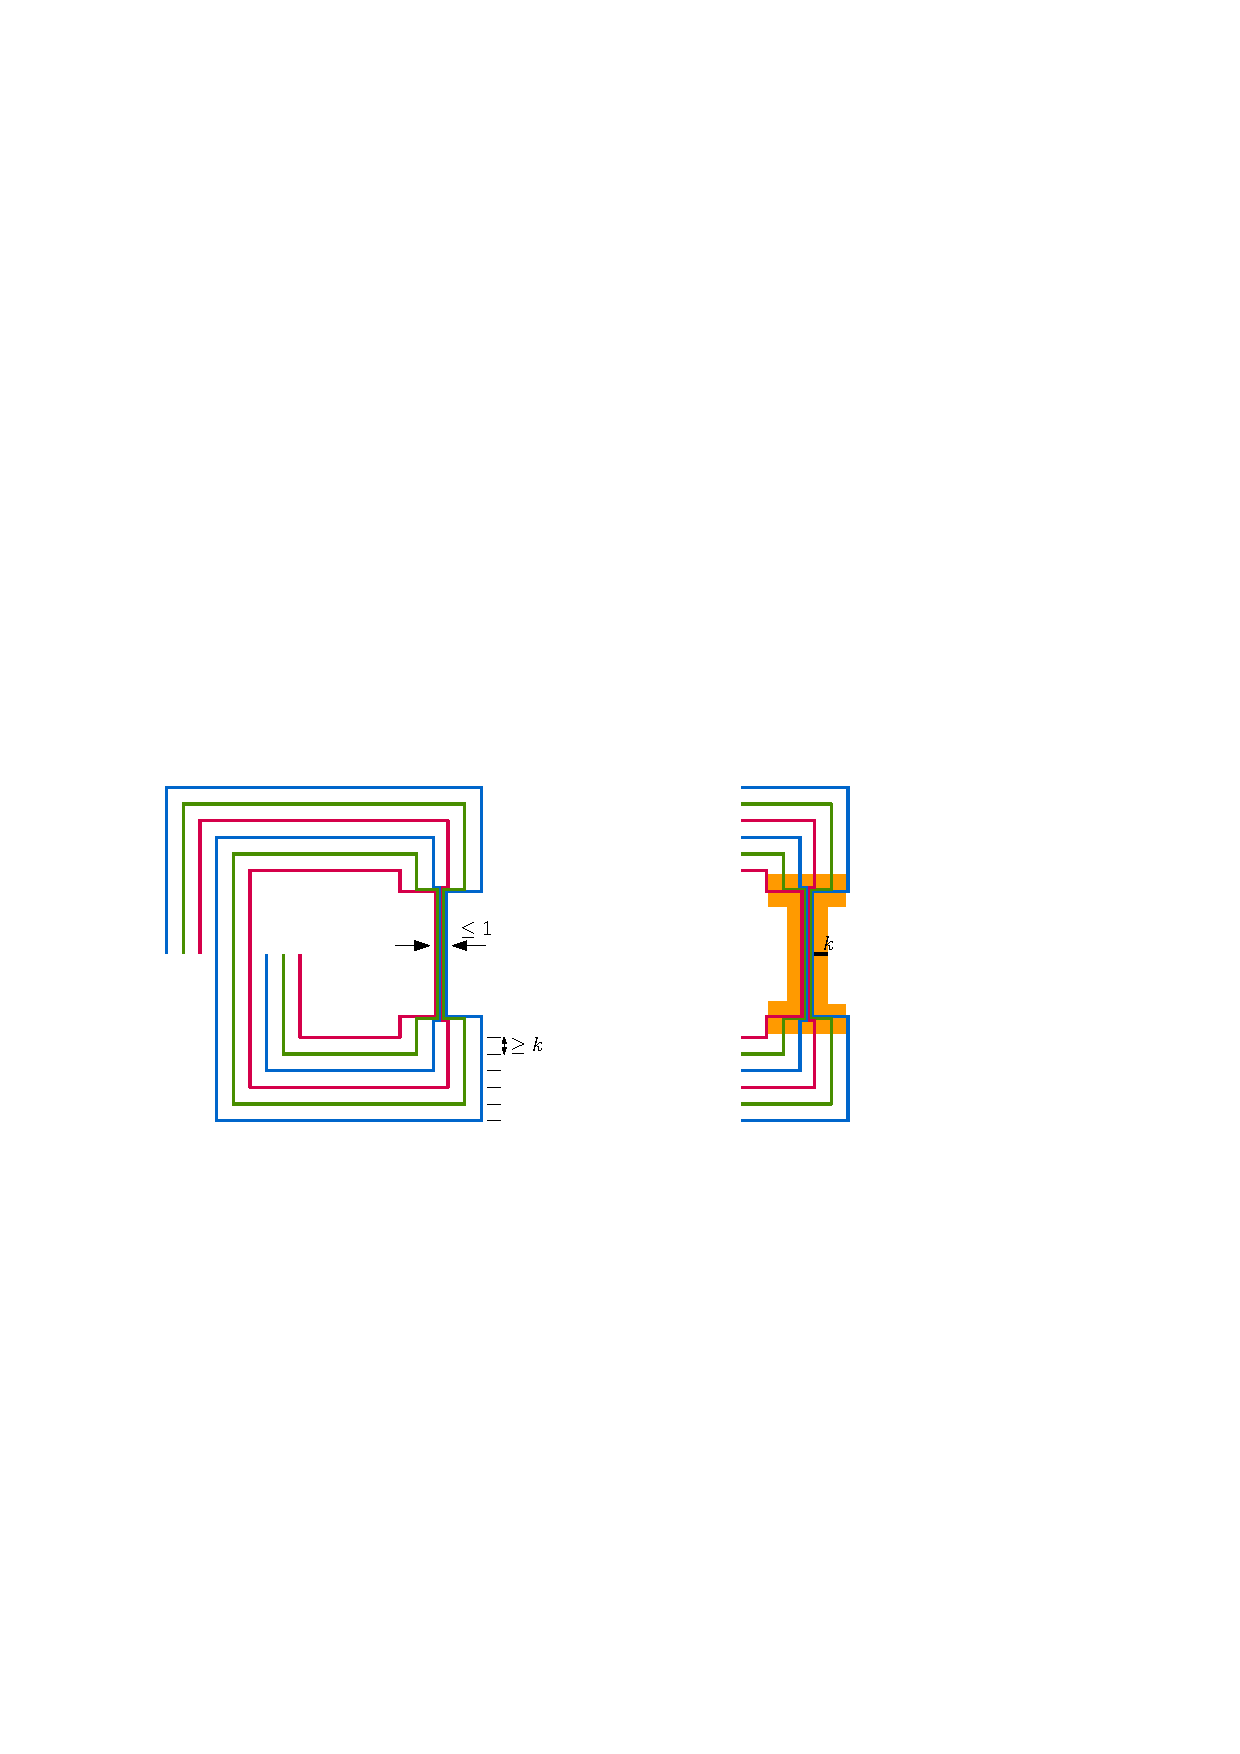
\includegraphics[scale=1]{Figures/arbitrary-lower-by-spirals.pdf}
\caption{The regions for $k=1$. The region $\ixi$ is highlighted in yellow.}
\label{fig:arbitrary-spirals}
\end{figure}

% Everything outside $\ixi$ can easily be drawn without much stretch.
% Also for everything outside $\mathcal{I}$, there is not much choice for the coloring (topologically). Area $\ixi$ is the problem here.
%Note that at the top and the bottom we have $3k+3$ "connections" each. In $\ixi$ the pixels are colored in $c_1$ (red), $c_2$ (green) and $c_3$ (blue) such that in the end, the three polygons $P_1$, $P_2$ and $P_3$ induced by the three colors are connected.

%Let $k\Xi$ be a superpixel grid of size $f(\ell)$ \jerome{to be determined} aligned like in Figure~\draw. The input polygons $R_i$ intersect all of the superpixels in $\ixi$. \jerome{take care to make a small wiggle in the corners of the $\ixi$ so that this holds.}
%Just outside of $\ixi$ the superpixels blibla \todo{insert coordinates} all need to contain the colors redorgreenorblue.

%Due to the choice of $\ixi$ we have that no pixel outside $\ixi$ and the loops is colored.
%Due to the choice of the size of $k\Xi$ we know that each pixel in any superpixel in the area highlighted in Figure~\draw is colored in the background color.
%We assumed that the similarity is bounded by $k$, which implies that there is a valid coloring $C$ with stretch at most $k$.

Let $H=(W, F)$ be the Reeb graph of the (disconnected) regions $R=(R_1\cup R_2\cup R_3)\cap \ixi$.
Note that $H$ is plane. Additionally $W$ contains $3\cdot k + 3$ vertices $W_t=\{r_1, g_1, b_1, r_2,\dots, r_{k+1}, g_{k+1}, b_{k+1}\}$ that correspond to the intersections of the regions $R_1$, $R_2$ and $R_3$ and the top of $\ixi$. The names of the vertices indicate the color of the polygon. The vertices are sorted from left to right.
Similarly $W$ contains $3\cdot k + 3$ vertices $W_b=\textbf{}\{r'_0, g'_0, b'_0, r'_1,\dots, r'_k, g'_k, b'_k\}$ that correspond to the intersections of the regions $R_1$, $R_2$ and $R_3$ and the bottom of $\ixi$.
Now if two vertices $r_i$ and $r_j$ are connected within $H$, then no vertex $g_e$ or $b_f$ that is between $r_i$ and $r_j$ can be connected to a vertex of $W_b$. Note that there are always at least two vertices of different color between two vertices of the same color in $W_t$.
Similarly we have that if two vertices $r'_i$ and $r'_j$ are connected, then the vertices $g'_e$ and $b'_f$ between $r'_i$ and $r'_j$ are not connected to any vertex of $W_t$.
And the same also holds for vertices of different color.

Now let $E$ be a red connected component in $H$. Let $\{r_{i_1}, r_{i_2}, \dots, r_{i_e}, r'_{j_1}, \dots, r'_{j_f}\}$ be the members of $E$ that are in $W_t\cup W_b$, with $i_s<i_t$ and $j_s<j_t$ for $s<t$. We say that $E$ contains $e-1$ \emph{top brackets} and $f-1$ \emph{bottom brackets}. If either $e$ or $f$ is non-zero, we say that $E$ contains a \emph{top-bottom connection}. We extend this definition to blue and green connected components.

We know that when we remove $\ixi$ from the regions three $R_1$, $R_2$ and $R_3$, we obtain $3k+6$ regions. Therefore within $\ixi$ at least $3k+3$ connections (brackets and top-bottom connections) need to be made.
% This means that the connections within $\ixi$ must
Now let $x$ (resp.\ $y$) be the number of top (resp.\ bottom) brackets over all connected components in $H$. Additionally let $z$ be the number of top-bottom connections over all connected components in $H$.
We already established that for each bracket there are at least two vertices of different color that can not be within a connected component with a top-bottom connection.
\jerome{Should we somehow mention that this also extend to nested brackets or is that already implied? I have the complete proof that $z\leq 3 k +3 -3x$ written on paper.}
In addition to that we know that a bracket connects two vertices, which means that not both of them can have a top-bottom connection at the same time.
If there are no brackets we know that $z\leq 3 k +3$.
Overall this means that we have less than $3k+3 - 3x$ and less than $3k+3 - 3y$ top-bottom connections.
% , i.e., $z\leq 3\min(k+1 - x, k+1-y)= 3(k+1 - \max(x,y))$.
% However we have that each bracket and each top-bottom connection connects two connected components. So we need $x+y+z\geq (3k+6)-3=3k +3$ connections.
Without loss of generality we can assume $x\geq y$.
It follows:
\begin{align*}
    3k+3\leq& x+y+z\\
    \leq& 2x + 3k+3 - 3x \\
    \iff& \\
    x&\leq 0
\end{align*}

As we have $0\leq y\leq x$, this means that the number of brackets is zero. This implies we have $3k+3$ top-bottom connections.

However all the connections must be within distance $k$ of the middle pixel. \todo{define middle pixel}. It is impossible to rout $3k+3$ connections using only $2k+1$ pixels. \jerome{rephrase previous sentence}
Contradiction

\end{proof}

% This implies that for three or more polygons the best fitting grid polygons have unbounded..... I do not know how I can phrase this ...

% section arbitrary (end)


\section{Conclusion} % (fold)
\label{sec:conclusion}

Open Questions that can be still researched:
\begin{enumerate}
	\item fat non-convex polygons for interesting fatness definitions. Because for some of them Theorem~\ref{thm:unbouded} holds.
	\item How about two polygons in the general setting? This would create an interesting comparison to either the one polygon or the three polygon cases where one is easy and one is unbounded.
	Solved reading: The Painter’s Problem: Covering a Grid with Colored Connected Polygons
	\item Can we give an algorithm for a stretch depending on the complexity of $A$, i.e., number of vertices, rotation number, \dots?
	\item We can also do a set of point regions and one more arbitrary region without upsetting the $O(\sqrt{m})$ bound. Is this also true for two arbitrary regions with $m$ point regions? Is it also true for convex regions and one or two arbitrary regions? And fat convex?
\end{enumerate}

% section conclusion (end)

\newpage
\appendix



\section{Write-up from Ivor for: Holes are Points}



Assume that all the holes are points. In that case we can create a pixel projection $B$ with a $\Theta(\sqrt[]{md})$ symmetrical Hausdorff distance to $A$. This projection is also used in the next section where regions are convex $\beta$-fat regions.  The lower bound for this variant is obtained in the following way: let there be $m$ holes in one pixel of diameter $d$. Then because the holes need to be disjoint, we need to expand all of $A$ by at least a factor $2\sqrt[]{m}d$ in both directions to allow each hole to have a single disjoint pixel.

\begin{figure}[H]
\centering
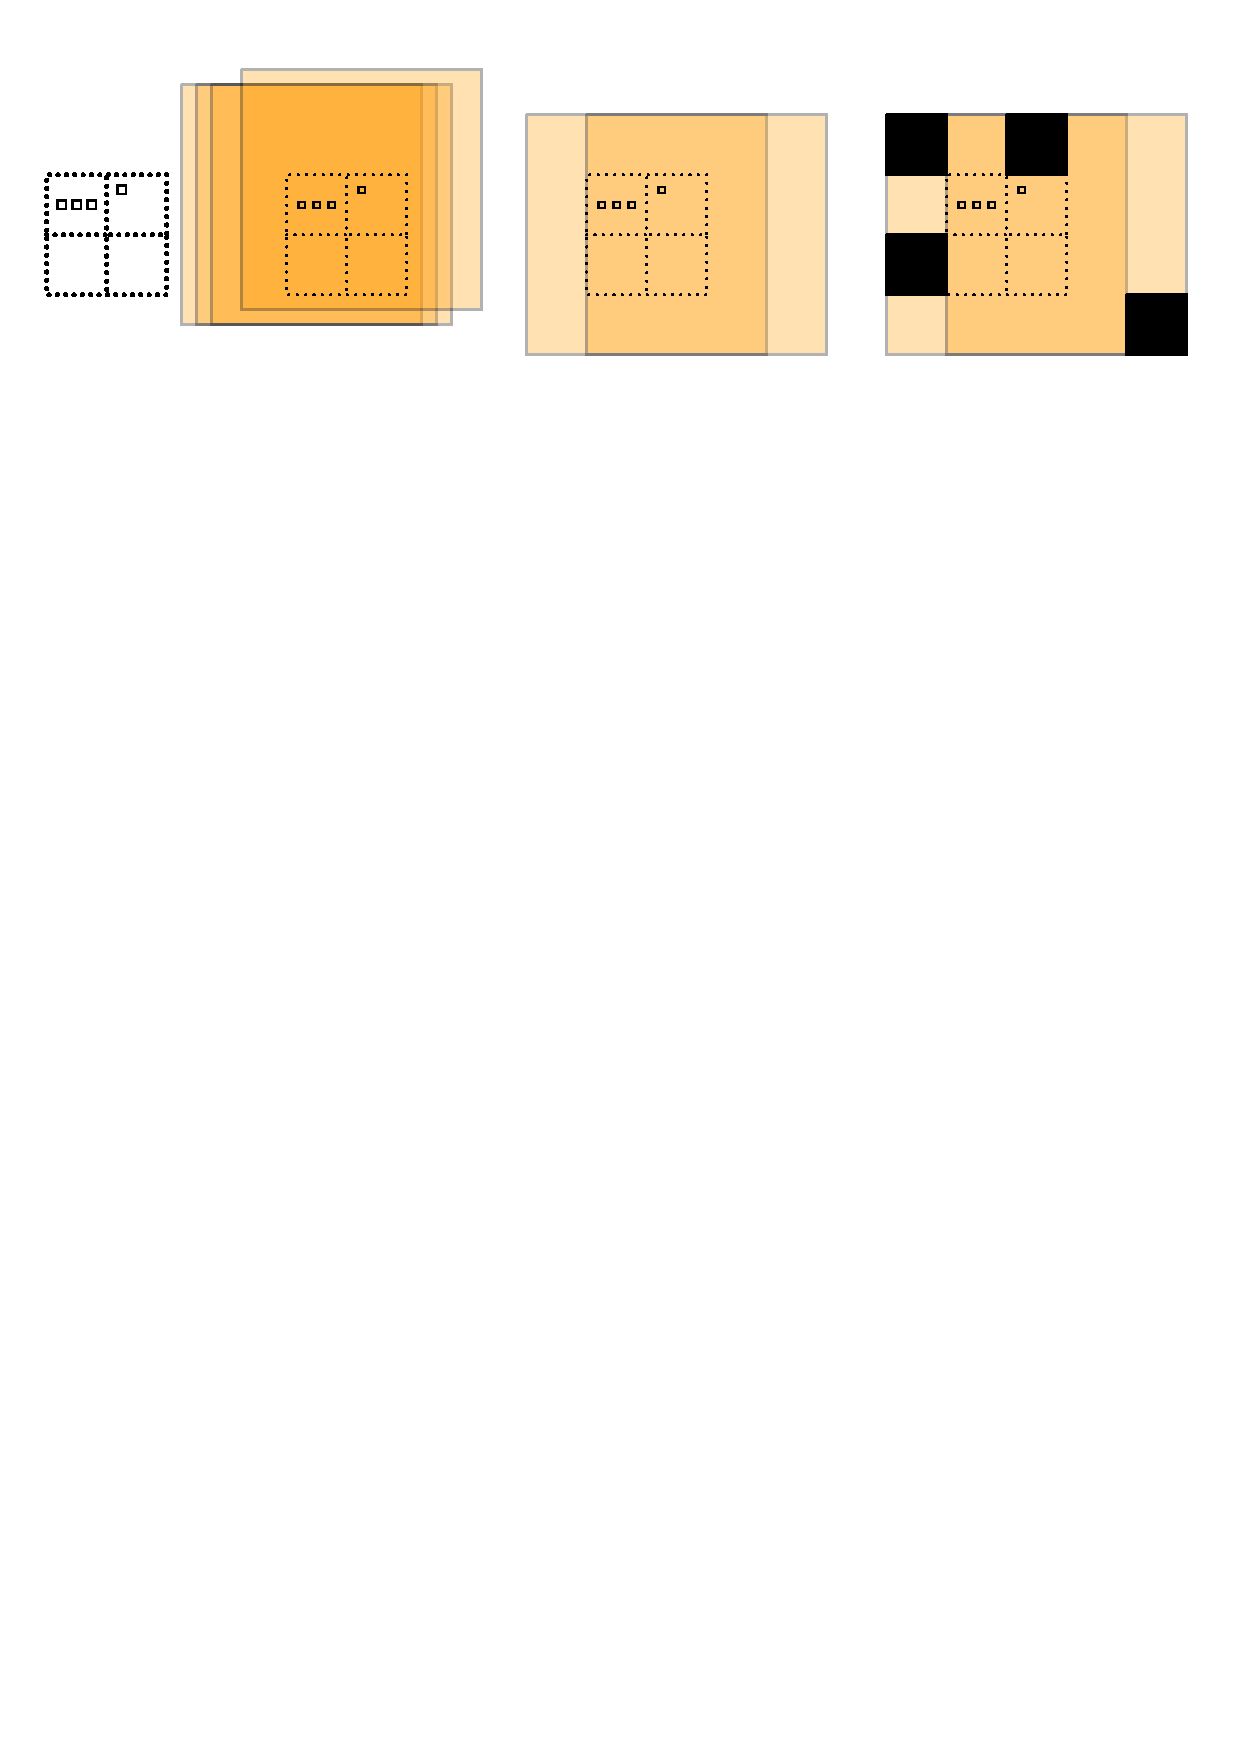
\includegraphics[width=\textwidth]{Figures/pointprojection.pdf}
\caption{The four steps of the point projection $f$. Left we see $m=4$ points in two pixels with diameter $d$. The second frame shows all the non-translated regions $D_h$ with diameter $2\sqrt[]{m}d$. The third frame shows their translation, observe that holes in the same pixel always get assigned the same region $D_h$. The fourth frame shows an arbitrary assignment of holes to pixels in their regions.}
\label{fig:pointprojection}
\end{figure}


Given our object $A$ we can create a valid projection with a symmetrical Hausdorff distance to $B$ as follows: we assign to each hole $h \in H$ an axis-parallel square $D_h$ with diameter $2\sqrt[]{m}d$. We then align all the regions $D_h$ in the same way, in Figure \ref{fig:pointprojection} we align them to assign them to the left-bottom corner of each $D_h$ with the left-bottom corner of the pixel that contains the left-bottom corner of $D_h$. Lastly we iteratively assign each hole to a pixel in $D_h$ which is disjoint from any assigned pixel. There must always be such a pixel, because there are $4m$ pixels in each $D_h$ and there are only $m$ holes. This process gives a projection $f$ on $H$ with a symmetrical Hausdorff distance of at most $2\sqrt[]{m}d$ and Lemma \ref{lemma:expand} proves the rest.



\section{Write-up from Ivor for: Holes are Convex and Fat}



Recall that a region $B$ is $\beta$-fat if there exists an inscribed circle $I(B)$ and a enclosing circle $E(B)$ such that $\frac{|E(B)|}{|I(B)E} = \mathcal{O}(\beta)$.

Let the holes all be convex $\beta$-fat regions of arbitrary size. The projection for this case has a lower bound of $\Omega(\sqrt[]{m}d$ because the proof from the previous section can immediately be applied. The projection that realizes this lower bound borrows concepts from our previous projection. There we assigned to each region a ``super pixel'' $d_h$ with diameter $2\sqrt[]{m}d$. Instead of giving each hole a super pixel and aligning those with the grid, we first create aligned super pixels and assign our holes to those. We define $G$ be an arbitrary grid of super pixels $D$ with diameter $2\sqrt[]{m}d$ aligned with the pixel grid.

\begin{observation}
\label{obs:covering}
Observe that if any hole $h \in H$ which is $\beta$-fat and convex has a diameter greater than $\mathcal{O}(\sqrt[]{h})$ then $h$ has to cover at least one super pixel in $G$.
\end{observation}

\begin{figure}[H]
\centering
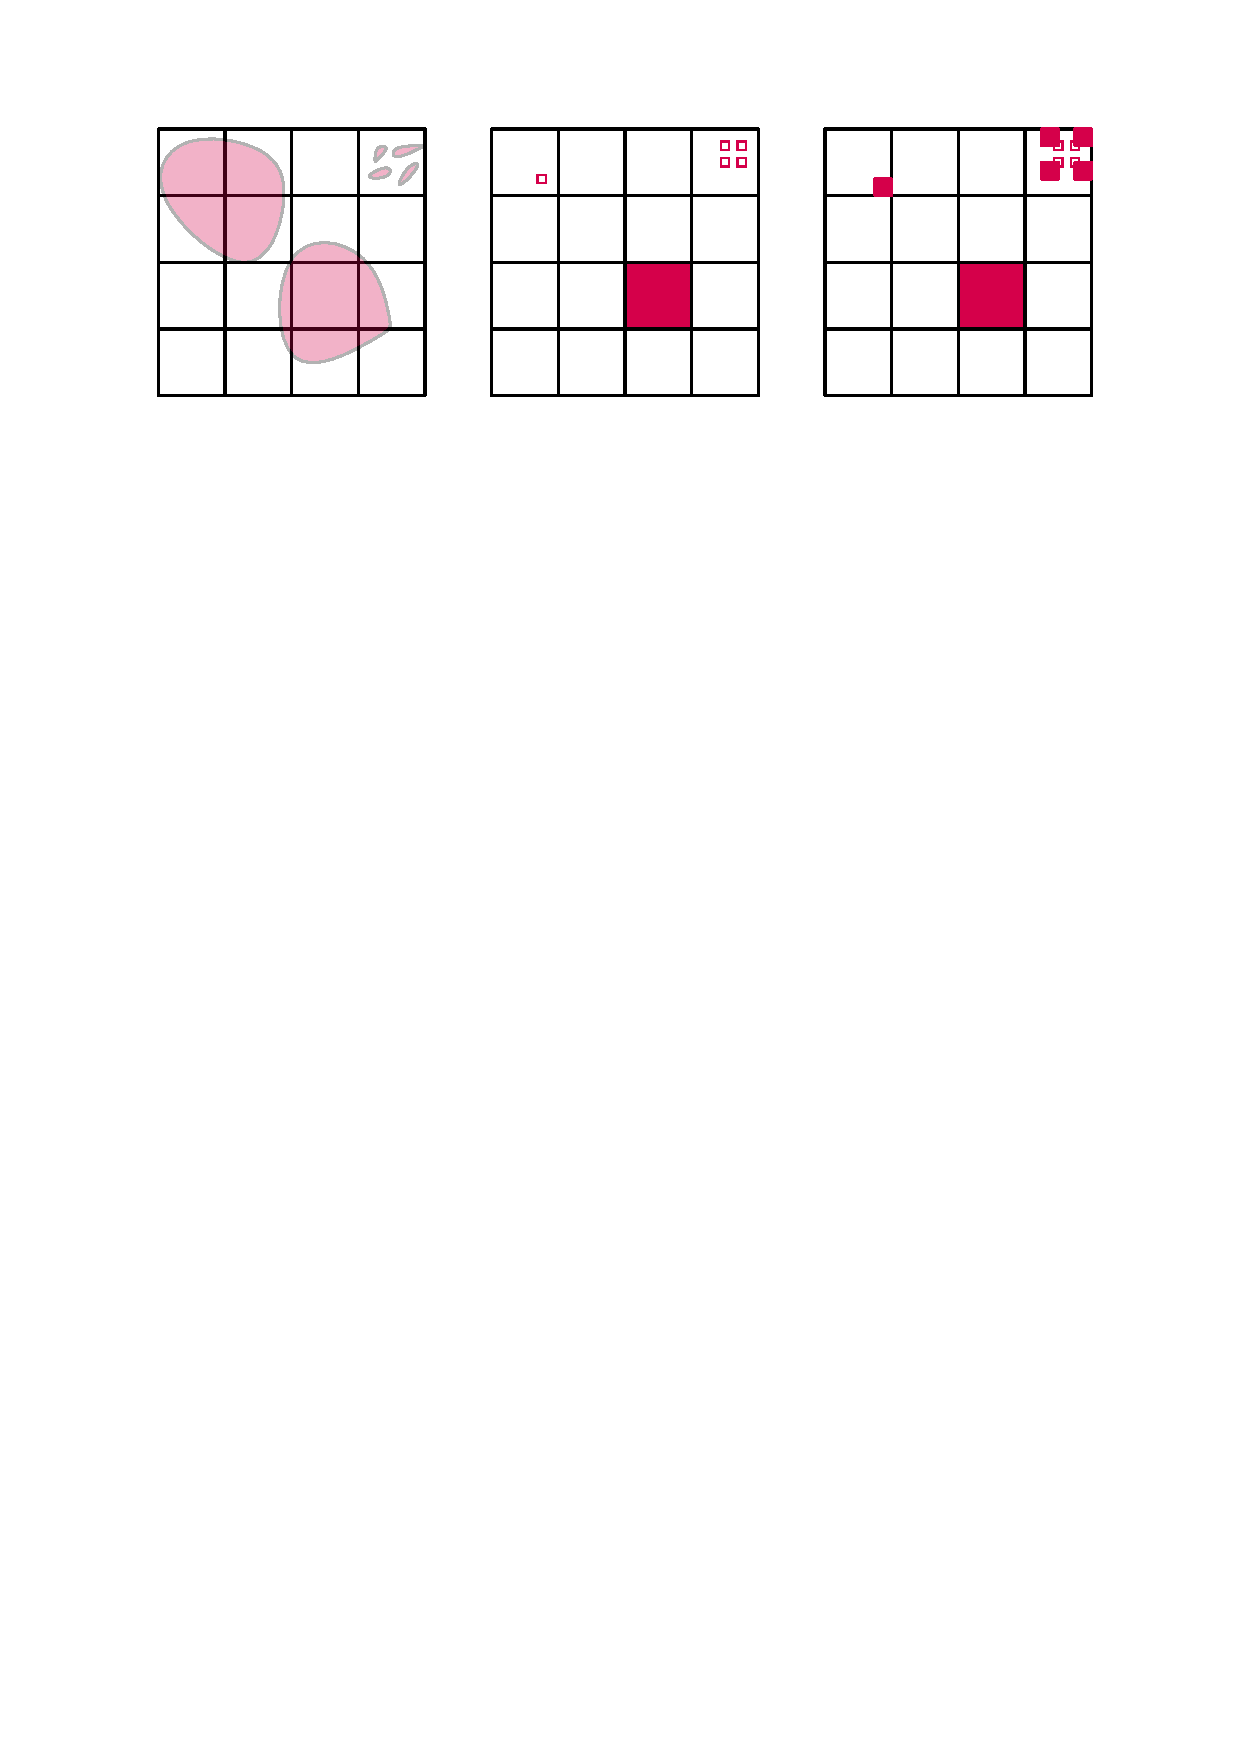
\includegraphics[width=\textwidth]{Figures/fatprojection.pdf}
\caption{The four three steps of the $\beta$-fat projection $f$. Left we see $m=6$ $\beta$-fat holes in red and 16 super pixels with black borders. The middle figure is the projection $C$ where one region is collapsed to a super pixel and the remaining regions are collapsed to a point. The last figure shows the final projection $B$ where each remaining point is assigned a pixel which has a diameter which is $2\sqrt[]{6}$ times smaller than the super pixel. }
\label{fig:fatprojection}
\end{figure}


With this observation, we can make the following projection: if a hole $h$ covers at least one super pixel, we let $h$ cover all the super pixels that it covers. The remainder of their area we throw away and all the other regions get collapsed to their center point. Because of Observation \ref{obs:covering} this in-between-projection $C$ has a $\mathcal{O}(\sqrt[]{h}d)$ Hausdorff distance to $H$.
Just like in the previous section, we then assign each point to an arbitrary disjoint pixel in its super-pixel to create our valid projection $B$. The symmetric Hausdorff distance between $H$ and $C$ is $\mathcal{O}(\sqrt[]{h}d)$ and the distance $C$ and $B$ is $\mathcal{O}(\sqrt[]{h}d)$ so the symmetric Hausdorff distance between $H$ and $B$ must be $\mathcal{O}(\sqrt[]{h}d)$. See Figure \ref{fig:fatprojection} for an example.



\section{Write-up from Ivor for: Holes are Convex}



Let the holes have as their only requirement that they are convex. In that case we can immediately show that the projection has a lower-bound Hausdorff distance of $\Theta(md)$. The construction is shown in Figure \ref{fig:linesexample}. We would like to create a projection of any set of convex holes $H$ that implements this lower bound such that all the projected regions are orthoconvex.


\begin{figure}[H]
\centering
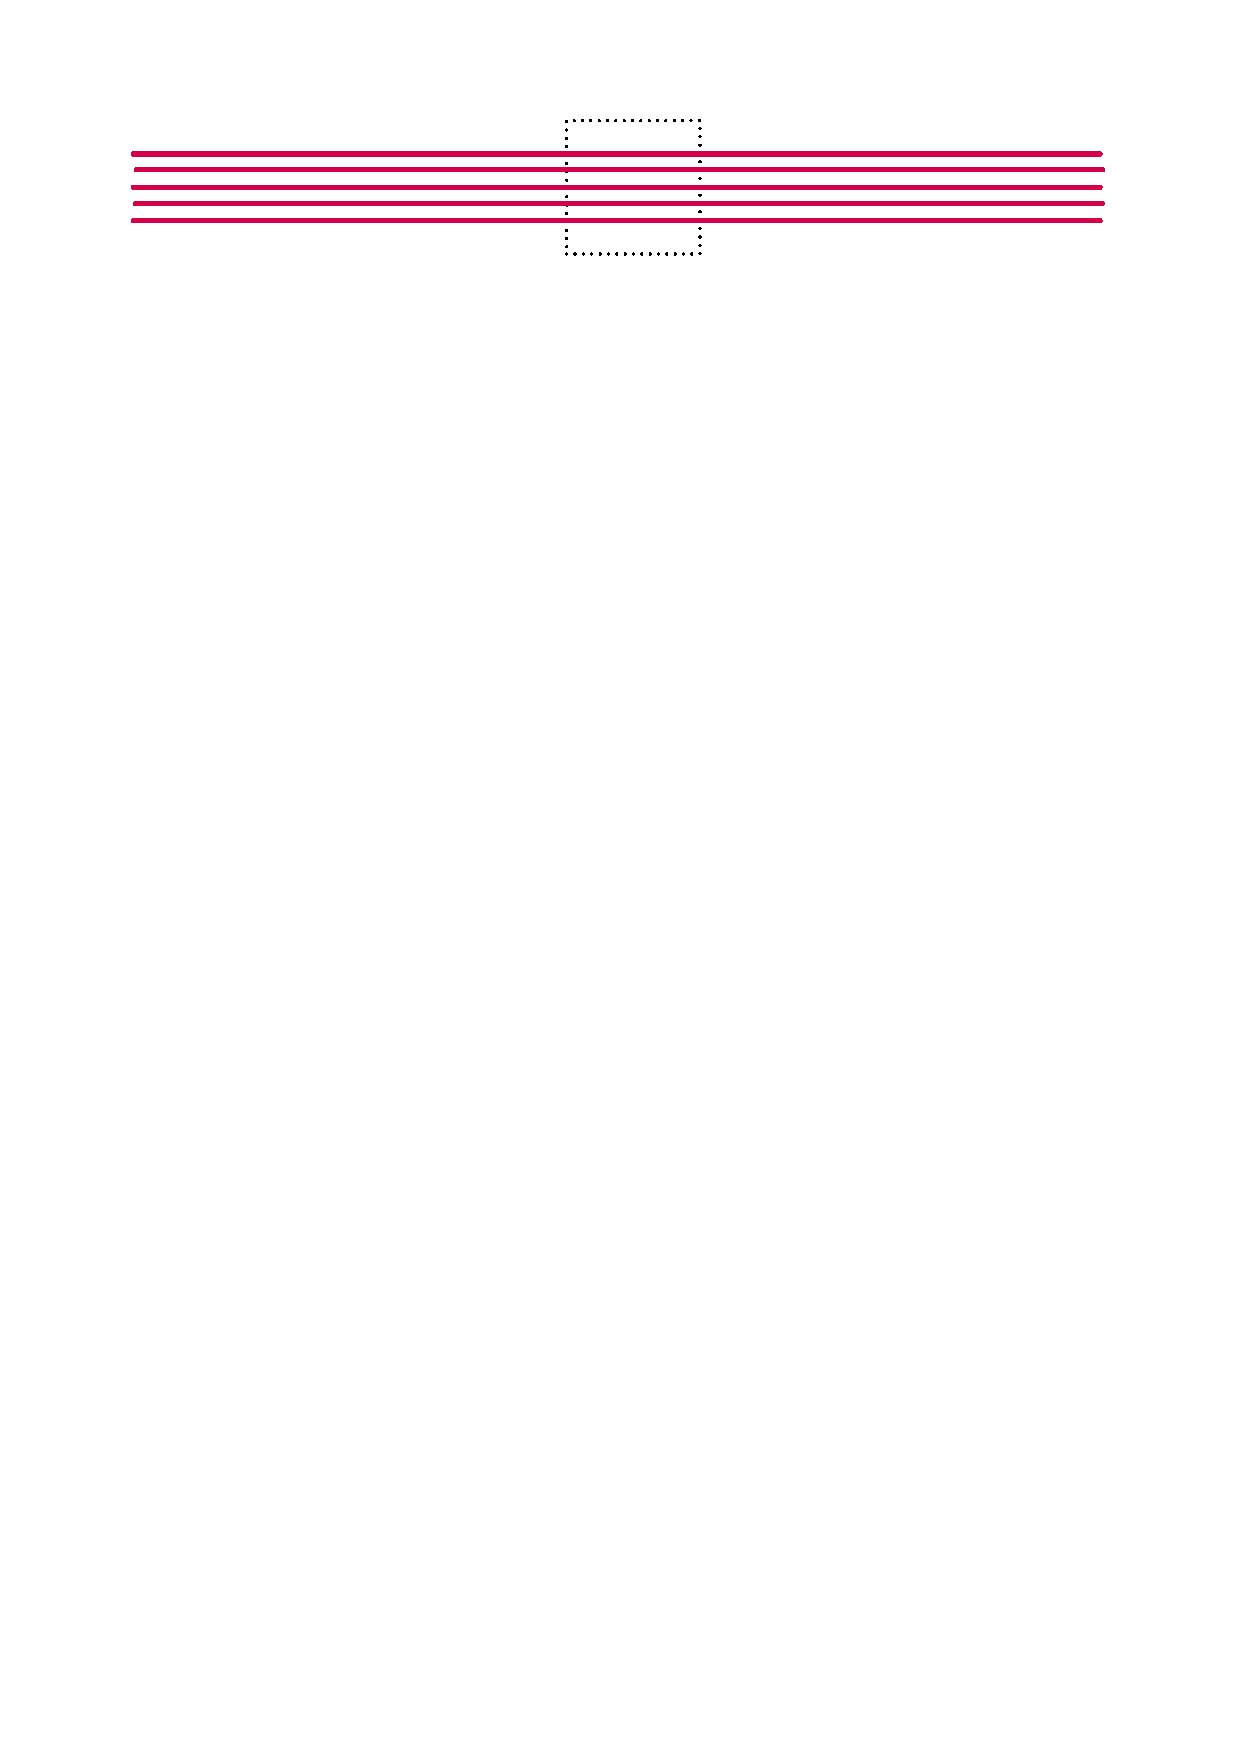
\includegraphics[width=\textwidth]{Figures/linesexample.pdf}
\caption{The dotted square is a pixel with diameter $d$. We can let $m$ vertical lines intersect the pixel. If their length is far greater than $md$, we can only project these regions to $dm$ disjoint lines of pixels, which means that the outer lines must have a Hausdorff distance of $\Theta(md)$.}
\label{fig:linesexample}
\end{figure}


\begin{observation}
Let $R_1,R_2 \in H$ be two convex regions. If there exists a horizontal line segment $l_1$ which intersects $R_1$ and $R_2$ such that on $l_1$, $R_1$ is left from $R_2$ then there cannot be another horizontal line segment $l_2$ which intersects $R_1$ and $R_2$ such that on $l_2$, $R_1$ lies to the right of $R_2$. A symmetrical property holds for vertical line segments if we look at which segment is higher.
\end{observation}

To explain our orthoconvex projection, we first introduce some notation: the observation allows us to create a partial order $P_x$ and $P_y$ based on intersections with horizontal and vertical line segments respectively. Let $G$ be a grid of super pixels with diameter $2md+1$ that covers $H$, we denote a superpixel as $D \in G$. We define $X_H$ and $Y_H$ to be two indexes on $H$ that respect the partial orders $P_x$ and $P_y$ respectively. For any $D \in G$ we denote $D[x,y]$ to be the pixel in $D$ that is the $2x+1$'th from the left and the $2y+1'th$ pixel from the top. The algorithm involves assigning super pixels and pixels in $G$ to holes $h$ and in the end connecting those holes.

\begin{enumerate}
%\item If a hole $h$ covers at least one super pixel $D \in G$, we assign all $D$ which are coved by $h$ entirely to $h$.
%\item If a hole $h$ covers no super pixel, then for each super pixel $D$ which is intersected by $h$ we assign $D[X_H(h), Y_H(h)]$ to $h$.
\item For each super pixel $D$ which is intersected by a hole $h$ we assign $D[X_H(h), Y_H(h)]$ to $h$.
\item For all holes $h$, we connect all assigned pixels with a horizontal and vertical line.
\item If a set of lines encloses a region, we fill that region.
\end{enumerate}


\begin{figure}[H]
\centering
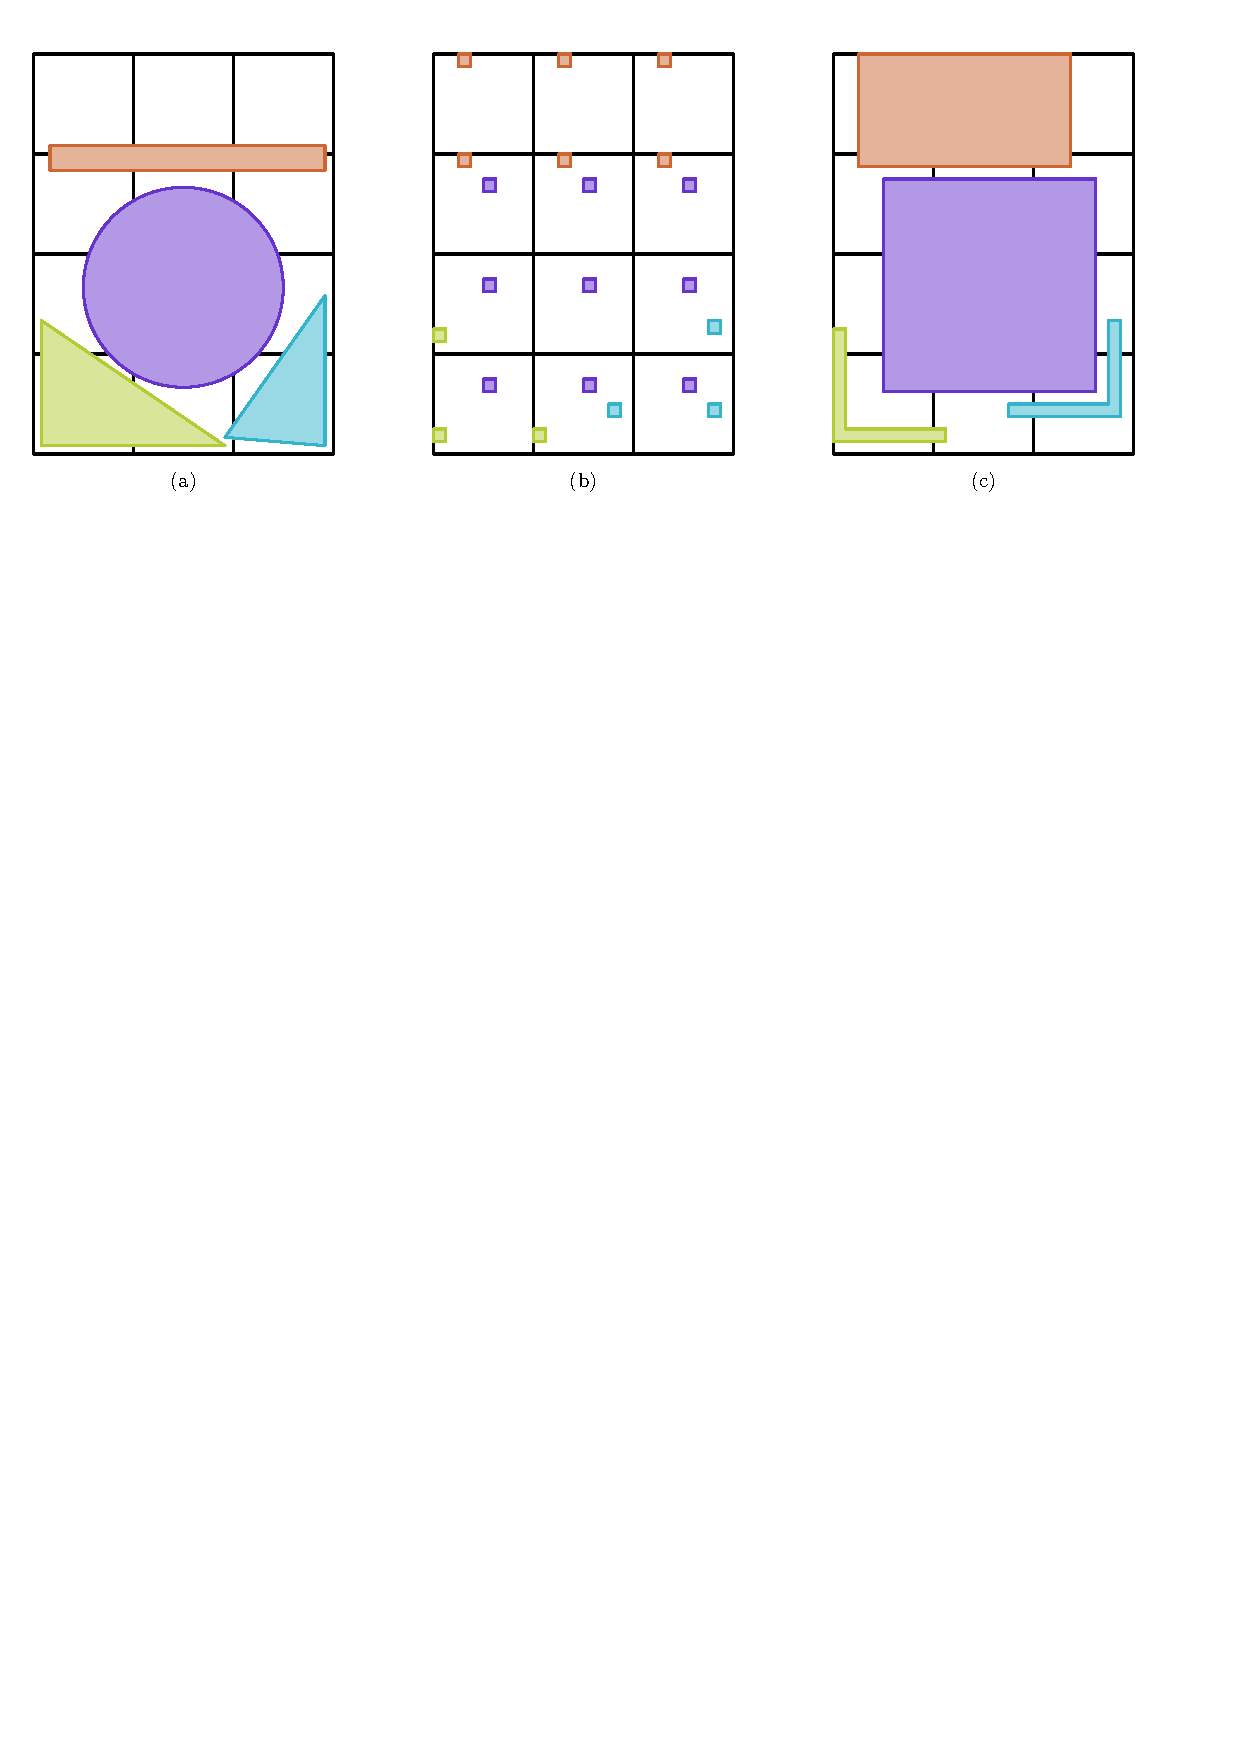
\includegraphics[width=\textwidth]{Figures/convexprojection.pdf}
\caption{Four regions that intersect three times four super pixels and the four steps of our algorithm. four.}
\label{fig:convexprojection}
\end{figure}

The result is clearly orthoconvex, since all assigned pixels are connected with horizontal and vertical lines and all enclosed regions are filled in. The result must also be disjoint: Any region that originally intersected a region which was filled in step 4 must originally have been to the left/right top/bottom of the region that filled a hole and thus is projected left/right above/below the filled region.



\section{Write-up from Ivor for: Old Algorithm on How to Draw Arbitrary Polygons}



We obtain the upper bound via a construction where we iteratively insert the $h$ holes into a grid in an arbitrary order.
Fix an index on the holes: $H := \{ R_1, R_2 ... h_h \}$ and fix a 2-dimensional grid $G$ with cell diameter $ d 2^{h+1}$ over $A$.
For each grid cell $\hfill\pix$ we check which holes in $A$ intersect $\hfill\pix$ and we mark $\hfill\pix$ with these holes.

\begin{observation}
If in our projection each hole $R_i$ is a connected tree which spans all grid cells marked by $R_i$ then the symmetrical Hausdorff distance is $\Theta(d2^h)$.
\end{observation}

\begin{definition}[The iteration invariant]
In our proposed algorithm. After inserting hole $R_i$, every hole $h_j$ with $j \le i$ is a spanning tree. Where the tree has as least one vertex in each cell marked by $h_j$ and edges between vertices are orthogonal.
\end{definition}


Our algorithm works as follows: We start by inserting $R_1$ as an orthogonal MST of the center points of all its marked cells. This is clearly possible and it maintains the iteration invariant.



For all remained holes $R_i$ we do the following:

\paragraph*{Step 1}
We start by adding a (orthogonal) closed face around each hole $h_j$ with $j < i$ in the following way:
For each hole $h_j$ with $j < i$, for each edge $(a,b)$ we add four vertexes: $x_a, y_a, x_b, y_b$.  $x_a, x_b$ and $y_a,y_b$ are always connected with an orthogonal edge. If $a$ is a leaf, then $x_a,y_a$ are connected with an orthogonal edge and the same holds for $x_b,a_b$. Else per construction these edges are connected to another vertex. This creates an orthogonal face around each hole $h_j$.
Lastly we glue the holes together in the following way: For every pair of edges of $R_i$, if they are parallel, their endpoints pairwise end in the same grid and there is no edge in between, we identify then with one another.

Each cell $\hfill\pix$ which is marked by $R_i$ and does not contain a vertex of $R_i$, we add a vertex of $R_i$ and we name these vertexes \emph{champions}. In the original drawing $\hfill\pix$ was intersected by $R_i$ and connected. This in particular means that at least one edge of $\hfill\pix$ was intersected by $R_1$. For these edges we add an orthogonal edge from the champion to the cell that shares the edge with $\hfill\pix$. The result is that $R_i$ is connected and that there is a vertex in each cell marked by $R_i$.
note that after step 1. The iteration invariant holds for all holes $h_j$ with $j < i$ but not for $R_i$. See Figure \ref{fig:cycle} for an example.

\begin{figure}[H]
\centering
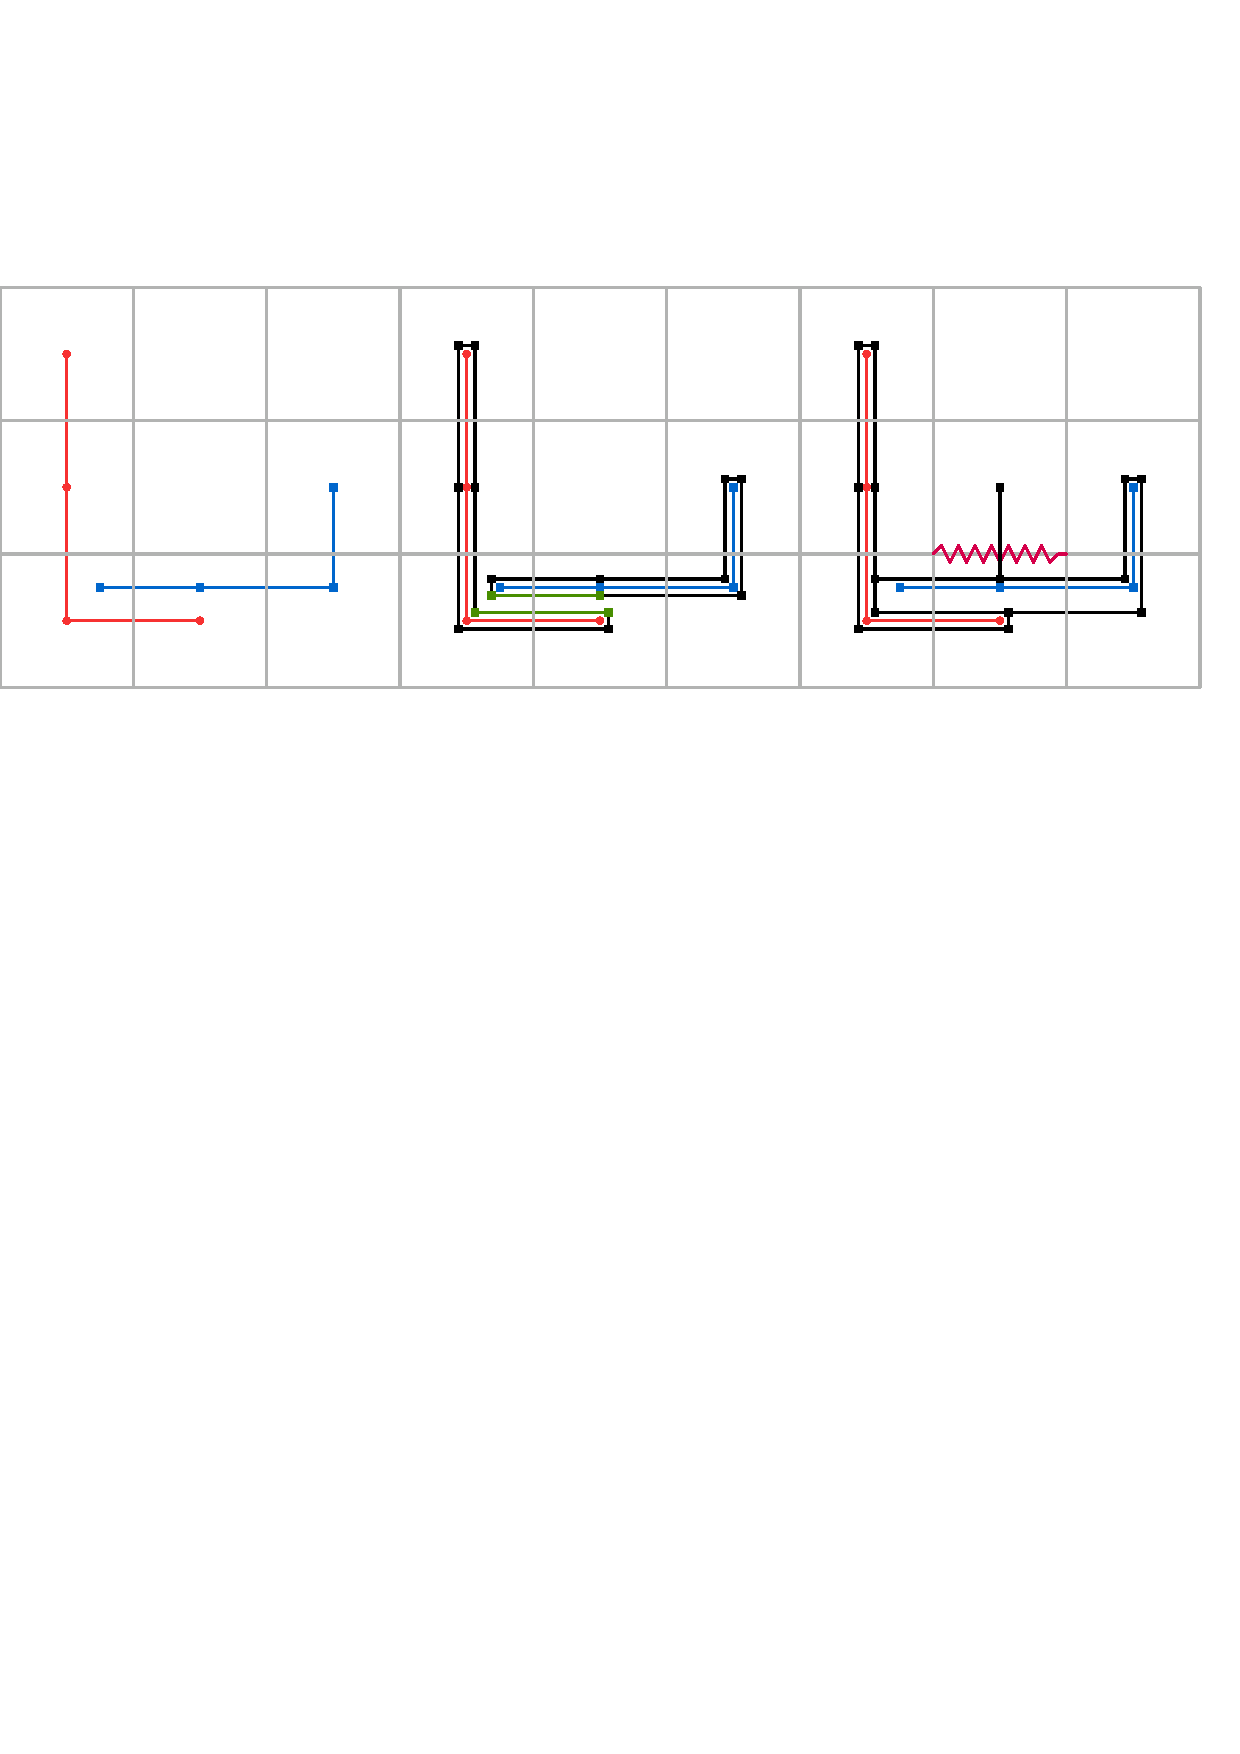
\includegraphics[page = 1]{Figures/cycle.pdf}
\caption{Left we see the result after inserting $R_1$ and $R_2$ in red and blue respectively. In the middle we see the two orthogonal cycles around $R_1$ and $R_2$. Note that the green edges can be identified to one another. The edge connected straight to the right is no candidate for gluing because the endpoints do not end in the same grid cells, so we get an extra }
\label{fig:cycle}
\end{figure}

\paragraph*{Step 2.}

In step 2. We delete all endpoints of $R_i$ which are in a cell that is not marked by $R_i$. We also delete all edges with less than 2 endpoints. All remaining vertices $x$ which used to have an outgoing edge and have lost it are marked \emph{broken.}

$R_i$ is now a collection of curves with three types of edges:

\begin{itemize}
\item Edges where all endpoints are regular (these are in the interior of a path). We call these \emph{regular edges}
\item Edges which end in a champion. We call these \emph{champion edges}
\item The case where at least one or two broken endpoints are involved but no champions. We call these \emph{broken edges}
\end{itemize}


\begin{observation}
after the gluing, each of $R_i$ is in at most 2 cycles.
\end{observation}
\paragraph*{Step 3.}

\begin{figure}[H]
\centering
\includegraphics[page = 2]{Figures/cycle.pdf}
\caption{ }
\label{fig:cycle2}
\end{figure}

\end{document}
